\begin{table}[htbp]
	\centering
	\caption{List of measurement equipment and components}\label{tab_appendix:KeSetUp}
	
	\begin{tabularx}{\textwidth}{lXXXX}
		Name 				& Brand	& Model & AAU-number									\\ \toprule \rowcolor{lightGrey}
		Oscilloscope	& Agilent & 54621D & 33941 	\\
		Powersupply	& Agilent & E3631A & 78577\\ \rowcolor{lightGrey}
		DC motor & Alsthom BBC & F9M2& 08339
	\end{tabularx}
\end{table}

\subsubsection*{Setup}
\autoref{fig:KeMeasurementSetup} shows a diagram and photo of the measurement set up
\begin{figure}[htbp]
	\centering
	\begin{subfigure}{0.50\textwidth}
		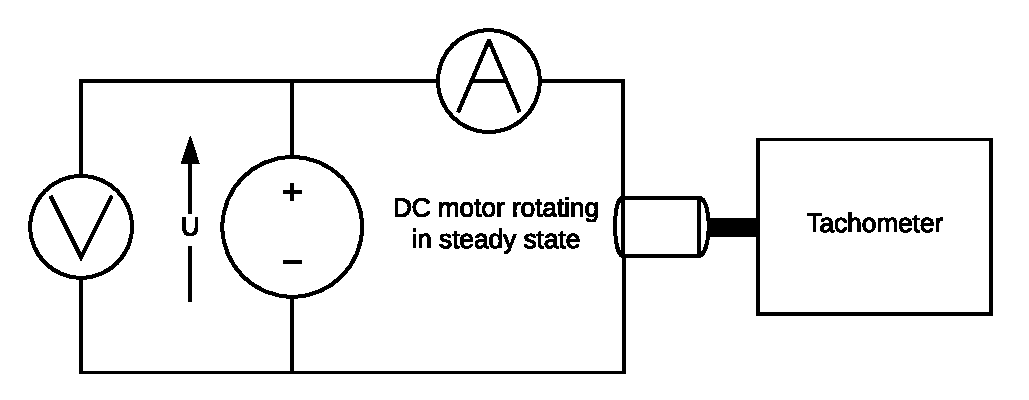
\includegraphics[width=\textwidth]{figures/appendix/Motor&GearTests/KeTestSetUp}
		\caption{Diagram of the set up.} \label{fig:KeMeasurementDiagram}
	\end{subfigure}
	\begin{subfigure}{0.40\textwidth}
		%\includegraphics[width=1\textwidth]{MotorImpedanceTest.jpg}
		\missingfigure{Picture of the setup}
		\caption{Picture of the set up.} \label{fig:KeMeasurementPictures}
	\end{subfigure}
	\caption{The measurement set up.} \label{fig:KeMeasurementSetup}   
\end{figure}

\subsubsection*{Method}
This test consists of having the motor shaft rotating in steady state while the voltage $U$ of the generator, the angular velocity $\omega$ of the shaft and the current $I$ are measured.

\subsubsection*{Raw data}
\autoref{tab:KeTest} has all the measurements done.


\subsubsection*{Data processing}

When the shaft is rotating in steady state as shown in \autoref{fig:KeMeasurementDiagram}, \autoref{eq:KeSetUpElec} can be derived.
\begin{equation}
U=K_e\omega+R_m I \addunit{\volt}
\label{eq:KeSetUpElec}
\end{equation}
\startexplain
\explain{$I$ is the current in the circuit}{\si{\ampere}}
\explain{$U$ is the generator's voltage}{\si{\volt}}
\explain{$K_e$ is the velocity constant of the motor}{\si{\volt\per\radian\second}}
\explain{$R_m$ is the internal resistance of the motor}{\si{\ohm}}
\stopexplain

From \autoref{eq:KeSetUpElec} \autoref{eq:KeForm} is obtained by isolating $K_e$.

\begin{equation}
K_e=\frac{U-R_m I}{\omega} \addunit{\volt\per\radian\second}
\label{eq:KeForm}
\end{equation}

\subsubsection*{Conclusion}

\autoref{fig:KeTest} plot the $K_e$ found for each measurement. The $K_e$ used in the model is average of these points. This gives $K_e=\SI{0.0343}{\volt\per\radian\second}$

\begin{figure}[htbp]
	\centering
	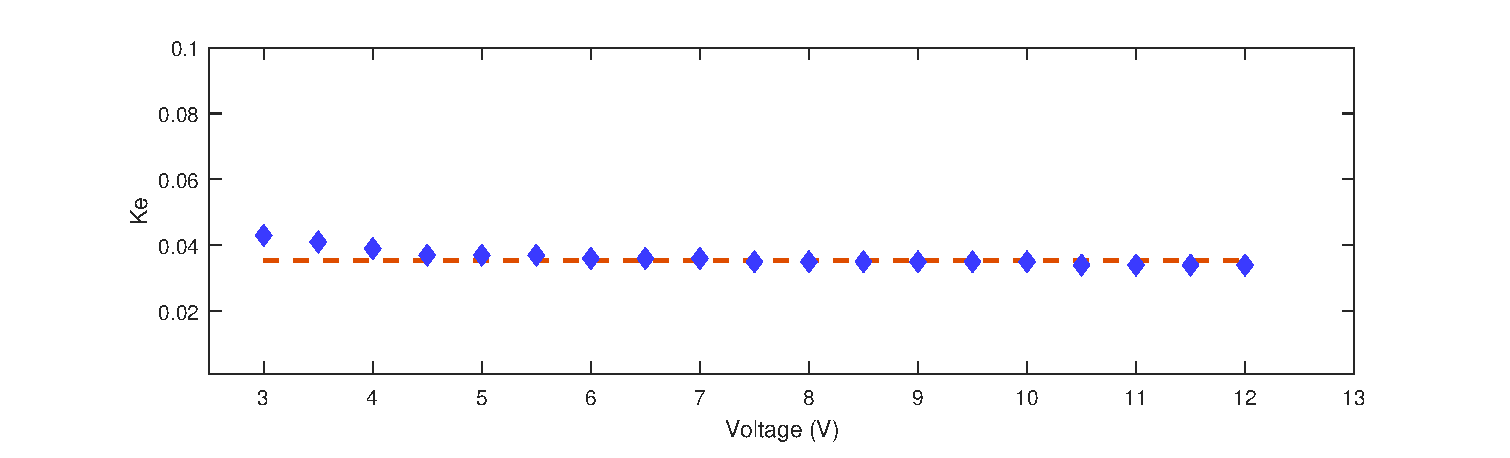
\includegraphics[width=1.1\textwidth]{figures/appendix/Motor&GearTests/PlotKe}
	\caption{Plot of $K_e$ found for each measures}\label{fig:KeTest}
\end{figure}